\chapter{\label{results}Results}
\thispagestyle{fancy}

\section{Current State}

\subsection{Init7 (Schweiz) AG}

Init7 is an \acrshort{ISP} since the year 2000. While it started with providing \acrshort{ADSL} service, they launched their fiber internet service
,,Fiber7'' in 2014 with competitive prices. Since then, the company has been expanding their geographical availability by
equipping an increasing amount of PoPs with their own infrastructure. The increase in infrastructure means that there is
an ever growing number of devices that have to be configured and managed. While they do employ automations, most of them
are implemented in the provisioning process. This would be mostly sufficient if they would only provide basic internet access,
as usually no configuration is needed to take a new customer online since the physical patching of the connection is done through
the owner of the fiber (usually power stations or Swisscom).

On the other hand, configuration is needed for a lot of \acrfull{B2B} products, as for example the following services:
\begin{itemize}
    \item Point-to-Point L2 connection: Enables the customer to create a layer 2 network across multiple sites.
      This can for example be implemented using a protocol like \acrshort{MPLS}.
    \item IP Transit: Enables the customer to directly connect to our core through \acrshort{BGP}.
    \item Business Internet Service: Very similar to a private service, but with the crucial difference that the customer
       uses \acrfull{CPE} which is managed and monitored by Init7.
\end{itemize}

In general, the business products also require Init7 to actively monitor status and quality. To be able to collect this data
both the access switch within the \acrfull{PoP} and the \acrshort{CPE} at the customer need to be configured accordingly.

While this thesis aims to provide a general solution for configuration, in order to keep the scope managable, the focus
and evaluation is limited to the access layer of the Init7 infrastructure.
To get a basic understanding of the Init7 infrastructure, a very simplified diagram is shown in [fig]. The \acrfull{IGP} used is
\acrshort{OSPF} and is split in two main parts. The core network ecompasses a cross-connected mesh of routers which are spread all
over the world. All interconnects and peerings to ISPs, customers and internet exchanges take place there. 

\begin{figure}[h]
  \centering
  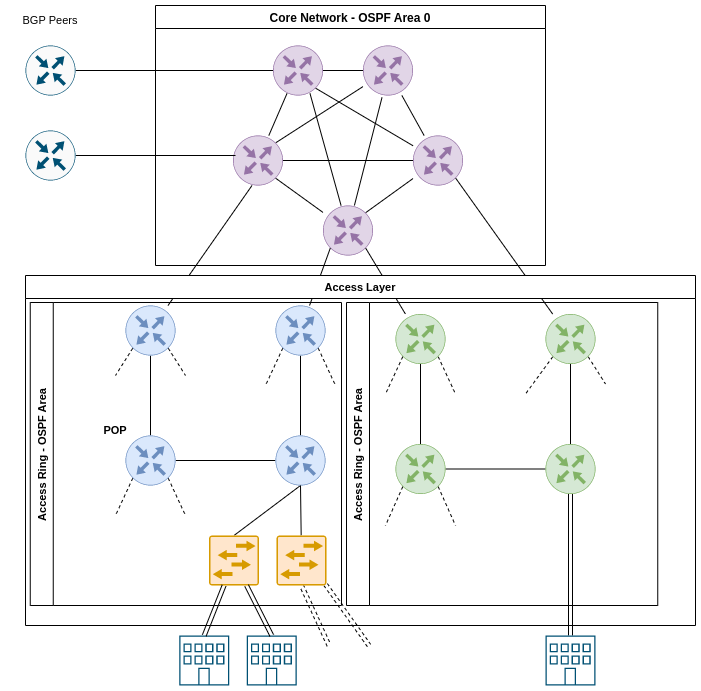
\includegraphics[width=0.7\textwidth]{Init7-Infrastructure}
  \caption{Init7 Topology}
  \label{fig:topology}
\end{figure}

TODO: Explain Access Layer


\section{Requirements Analysis}

\section{Application structure / Architecture}

To bridge the gap between the inventory management provided by NetBox and communicating with the actual hardware,
the solution is divided into layers.
In order to facilitate authentication and authorization there is the ,,Credential Access Manager'' which communicates
with an external credential store. The access manager provides a user interface to enter and manage credentials, as well
as restricting who has access to these credentials by integrating into the NetBox permission system.
The ,,Device Context Provider'' enables a user to define what information for a specific device shall be pulled.
Using the existing GraphQL API provided by NetBox, the user can easily identify what information is available and how it is
accessed. After the context data is defined it will subsequently be used in the ,,Configuration Template Editor''
where the user writes a template using the previously defined context data. This template can then be applied to
a class of devices utilizing constraints such as tags or locations.
Lastly, the ,,Configuration Transport'' module pulls the configuration template and the credentials for a specific device
and pushes it to the actual device.

\subsection{Credential Access Manager}



\subsection{Device Context Provider}

\subsection{Configuration Template Editor}

\subsection{Configuration Transport}



\section{Scenarios}

The following sections describe three chosen real-world scenarios within Init7.
More specifically, they are services which can be ordered by customers and also
require some manual work by network engineers in the current process.

The goal is to show how manual labor can be replaced or supported by the
created NetBox plugin.

\subsection{Fiber7}

Fiber7 is Init7's flag-ship product in the private consumer space,
providing consumers a \acrshort{P2P} fiber-optical connection directly into
Init7 infrastructure. Since this is the most commonly sold product by Init7
it is already one of the most streamlined processes throughout the department
with work being largerly automated.

\begin{figure}[h]
  \centering
  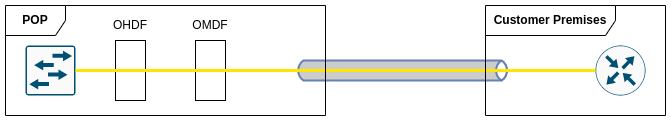
\includegraphics[width=\textwidth]{P-Fiber7}
  \caption{Fiber7 Service Diagram}
  \label{fig:fiber7}
\end{figure}

When the work-order arrives at the network engineer, it has already been decided
or defined at which \acrshort{POP}, network switch and interface the customer
will be connected to. The engineer will then go through the following process:

\begin{enumerate}
  \item A new service configuration ticket arrives
  \item Verify that there is no other active use on the chosen interface
  \item Apply the default configuration profile for Fiber7 private customers on the interface
  \item If the customer requested a static IP address, configure it on the DHCP server
  \item If the customer requested a prefix, configure it on the router connected to the switch
  \item If the customer does not specify a specific service activation date, enable the switchport
  \item Update NetBox with the performed configuration
  \item Update the service configuration ticket
\end{enumerate}

While the process might have seven steps, usually not all of that work is required.
When choosing the interface for the new service, it is verifed through the \acrshort{OSS}
that the port has no other active use.
Interfaces have the Fiber7 private customer profile configured by default
if it was previously unused or was previously used for the same service,
rendering step 3 usually unnecessary.
Most commonly, customers do not request static IP addresses or prefixes as
they are an additional cost to the subscription and are only used by ,,power-users'',
rendering steps 4 and 5 unnecessary.

The key observation that can be made, is that there are multiple manual steps
which can be prone to mistakes, yet they are always performed the same way. This makes
them good candidates for automation. Thus the goal is to restructure the process
to the following:

\begin{enumerate}
  \item A new service configuration ticket arrives
  \item Within NetBox:
  \begin{enumerate}
    \item Set the service field on the interface to Fiber7
    \item 
  \end{enumerate}
\end{enumerate}

\cn{(above) list not complete}

\cn{Describe process to extract template information}

\cn{Describe verification}

\subsection{Business Optical Service}


\begin{figure}[h]
  \centering
  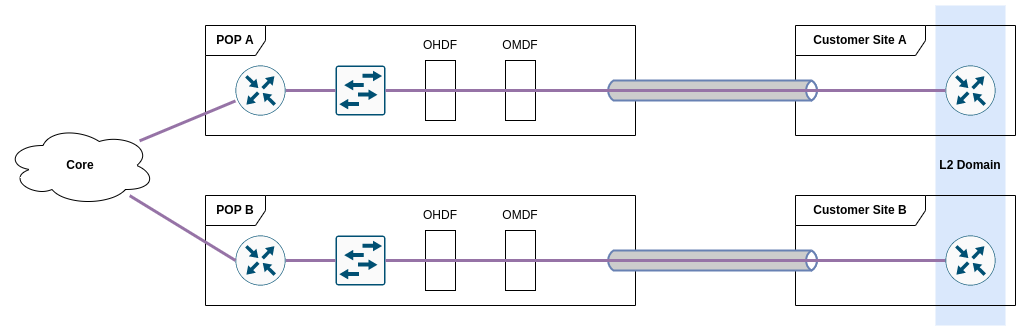
\includegraphics[width=\textwidth]{P-S2S}
  \caption{Business Optical Service Diagram}
  \label{fig:s2s}
\end{figure}

\cn{
 - B2B customer (standard)
  - Access Port with less configuration  \\
  - VLAN 600  \\
  - Static IP on router  \\
  - Static Route on router  \\
 - B2B customer (new)  \\
  - Trunk Port  \\
  - Allowed VLAN 600  \\
  - + same as standard?  \\
 - B2B Site-2-Site  \\
  - VLL through MPLS  \\

 - MikroTik ZTE  \\
 }